\documentclass[12pt, letterpaper]{article}

% ── Paquetes ─────────────────────────────────────────────────────────────────
\usepackage[utf8]{inputenc}
\usepackage[T1]{fontenc}
\usepackage[spanish]{babel}
\usepackage{geometry}
\usepackage{graphicx}
\usepackage{booktabs}
\usepackage{hyperref}
\usepackage{float}
\usepackage{caption}
\usepackage{subcaption}
\usepackage{enumitem}
\usepackage{parskip}
\usepackage{titlesec}
\usepackage{fancyhdr}
\usepackage{xcolor}
\usepackage{lmodern}
\usepackage{microtype}
\usepackage{csquotes}
\usepackage{listings}
\lstset{
  literate={á}{{\'a}}1 {é}{{\'e}}1 {í}{{\'i}}1 {ó}{{\'o}}1 {ú}{{\'u}}1
           {Á}{{\'A}}1 {É}{{\'E}}1 {Í}{{\'I}}1 {Ó}{{\'O}}1 {Ú}{{\'U}}1
           {ñ}{{\~n}}1 {Ñ}{{\~N}}1 {ü}{{\"u}}1 {Ü}{{\"U}}1
}

% ── Geometría ─────────────────────────────────────────────────────────────────
\geometry{
  top=2.5cm, bottom=2.5cm,
  left=2.5cm, right=2.5cm
}
\setlength{\headheight}{13.6pt}

% ── Hyperref ──────────────────────────────────────────────────────────────────
\hypersetup{
  colorlinks=true,
  linkcolor=black,
  urlcolor=blue!70!black,
  citecolor=black
}

% ── Encabezado / pie de página ────────────────────────────────────────────────
\pagestyle{fancy}
\fancyhf{}
\fancyhead[L]{\small Visualización de Datos -- Semestre I, 2026}
\fancyhead[R]{\small Tarea 1}
\fancyfoot[C]{\thepage}
\renewcommand{\headrulewidth}{0.4pt}

% ── Título de secciones ───────────────────────────────────────────────────────
\titleformat{\section}{\large\bfseries}{}{0em}{\thesection.\quad}
\titleformat{\subsection}{\normalsize\bfseries}{}{0em}{\thesubsection.\quad}

% ─────────────────────────────────────────────────────────────────────────────
\begin{document}

% ── Portada ───────────────────────────────────────────────────────────────────
\begin{titlepage}
  \centering
  \vspace*{1.5cm}

  {\Large\bfseries Universidad Técnica Federico Santa María}\\[0.3cm]
  {\large Departamento de Informática}\\[0.2cm]
  {\large Visualización de Datos -- Semestre I, 2026}

  \vspace{1.5cm}
  \rule{\linewidth}{0.5pt}\\[0.4cm]
  {\LARGE\bfseries Tarea 1: Herramientas de Visualización de Datos}\\[0.2cm]
  {\large Macrotema: \textit{Muerte} -- Suicidio a nivel mundial (1985--2015)}
  \rule{\linewidth}{0.5pt}

  \vspace{1.5cm}

  \begin{tabular}{ll}
    \textbf{Integrante 1:} & Alexis Mellis \\[0.2cm]
    \textbf{Integrante 2:} & Andres Aguila \\
  \end{tabular}

  \vspace{1cm}

  \begin{tabular}{ll}
    \textbf{Profesores:}  & José Luis Martí Lara \\
                          & Wladimir Ormazábal Orellana \\[0.3cm]
    \textbf{Ayudantes:}   & Fernanda Araya Zárate \\
                          & Carlos Arévalo Guajardo \\
  \end{tabular}

  \vfill

  {\large Fecha de entrega: 20 de abril de 2026}
\end{titlepage}

% ── Índice ────────────────────────────────────────────────────────────────────
\tableofcontents
\newpage

% ─────────────────────────────────────────────────────────────────────────────
\section{Introducción}

El presente informe corresponde a la Tarea 1 del curso de Visualización de Datos. El macrotema
elegido por el grupo es \textbf{Muerte}, con foco específico en las tasas de suicidio a nivel mundial
durante el período 1985--2016. El dataset utilizado fue obtenido desde Kaggle:

\begin{center}
  \href{https://www.kaggle.com/datasets/russellyates88/suicide-rates-overview-1985-to-2016}%
  {\texttt{suicide-rates-overview-1985-to-2016}}
\end{center}

Este conjunto de datos reúne información de múltiples países y permite analizar el fenómeno desde
distintas dimensiones: temporal, geográfica, demográfica y socioeconómica. En esta entrega analizaremos el dataset considerando todos los países.

% ─────────────────────────────────────────────────────────────────────────────
\section{Dataset y fuentes de datos}

\subsection{Descripción del dataset}

\begin{table}[H]
  \centering
  \caption{Principales variables del dataset.}
  \begin{tabular}{lp{9cm}}
    \toprule
    \textbf{Variable} & \textbf{Descripción} \\
    \midrule
    \texttt{country}        & País de registro \\
    \texttt{year}           & Año (1985--2016) \\
    \texttt{sex}            & Sexo (male / female) \\
    \texttt{age}            & Grupo etario (6 rangos) \\
    \texttt{suicides\_no}   & Número absoluto de suicidios \\
    \texttt{population}     & Población del grupo \\
    \texttt{suicides/100k pop} & Tasa por 100.000 habitantes \\
    \texttt{HDI for year}   & Índice de Desarrollo Humano \\
    \texttt{gdp\_per\_capita (\$)} & PIB per cápita en USD \\
    \bottomrule
  \end{tabular}
\end{table}

\subsection{Fuente}

\begin{itemize}[nosep]
  \item \textbf{Dataset principal:} Kaggle -- \textit{Suicide Rates Overview 1985 to 2016}.
        Disponible en: \url{https://www.kaggle.com/datasets/russellyates88/suicide-rates-overview-1985-to-2016}
  \item \textbf{Datos de origen:} United Nations Development Programme (UNDP), World Bank,
        World Health Organization (WHO) y Szamil (Kaggle).
\end{itemize}

% ─────────────────────────────────────────────────────────────────────────────
\section{Trabajo individual -- Integrante 1: Alexis Mellis}

\subsection{Criterios seleccionados}

\begin{enumerate}
  \item \textbf{Criterio A:} Evolución temporal de la cantidad global de suicidios.
  \item \textbf{Criterio B:} Distribución etaria de suicidios a lo largo del tiempo.
\end{enumerate}

\subsection{Justificación de los criterios}

El Criterio A permite observar la magnitud macro del problema, identificando rápidamente las tendencias históricas y los periodos de mayor crisis. 
Al centrarse en el volumen total, establece una base clara para evaluar el impacto del fenómeno a largo plazo. Por su parte, el Criterio B desglosa este volumen para 
evidenciar quiénes son los más vulnerables en cada periodo.

\subsection{Visualización 1}

\begin{figure}[H]
  \centering
  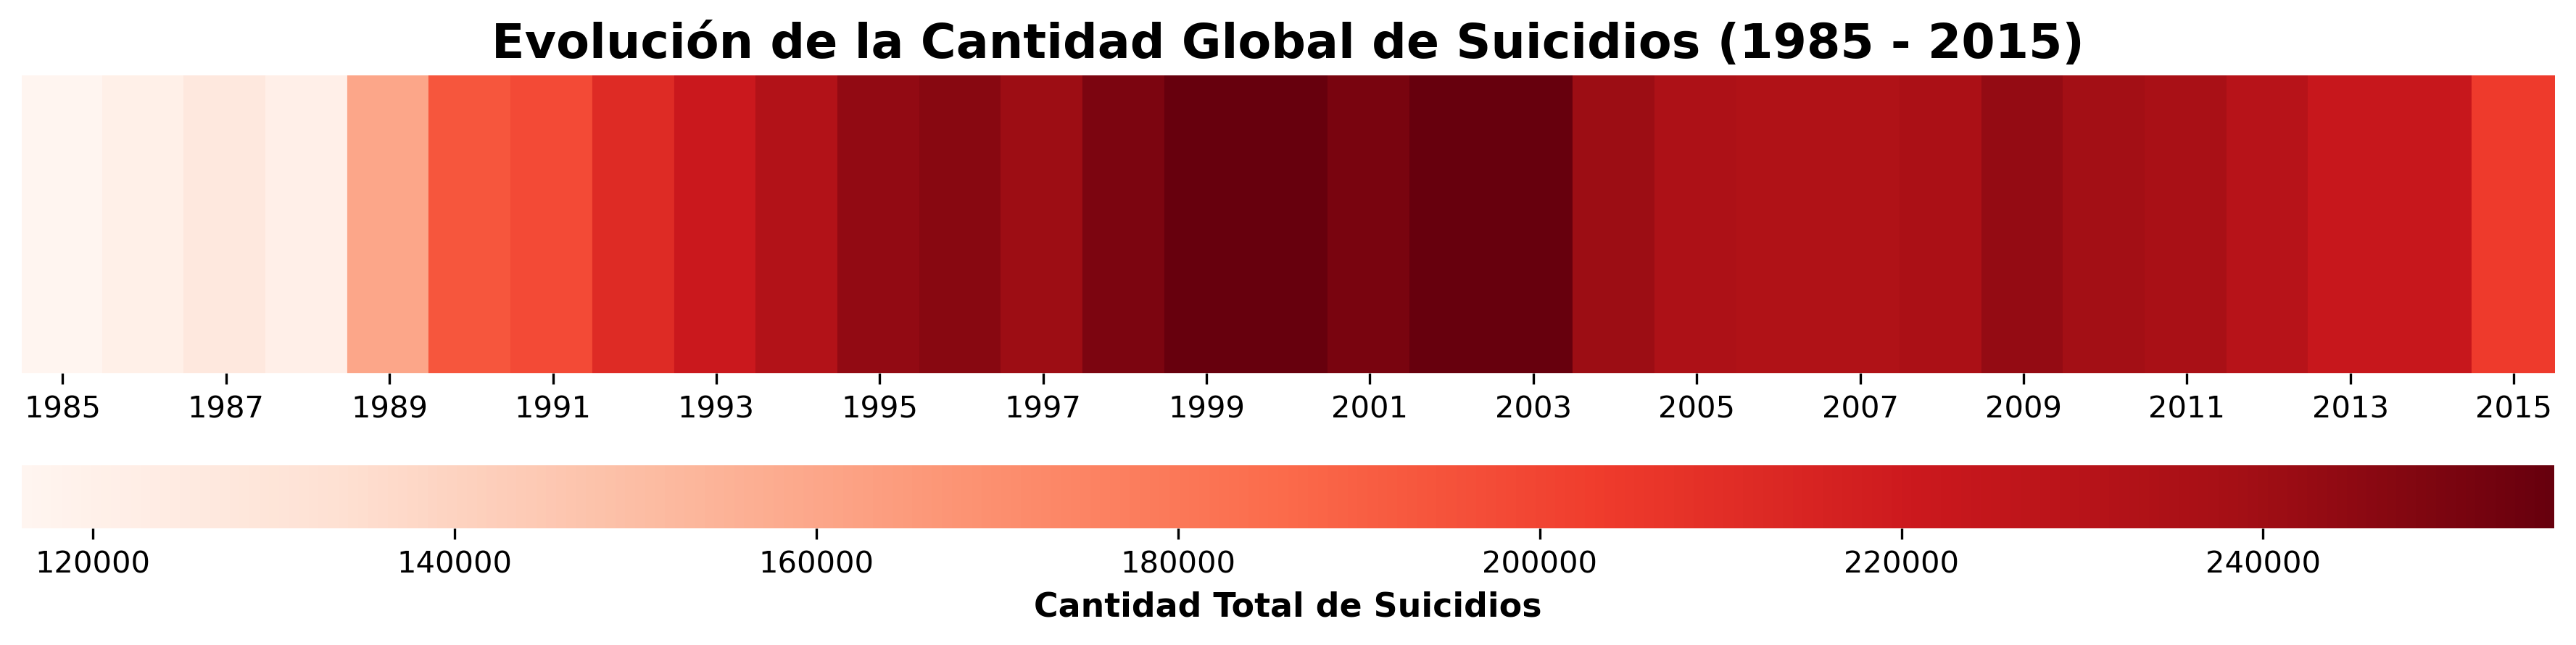
\includegraphics[width=0.85\textwidth]{figures/figure001.png}
  \caption{Evolución de la Cantidad Global de Suicidios (1985 - 2015). Fuente: Kaggle -- Suicide Rates Overview 1985--2016.}
  \label{fig:figure001}
\end{figure}

\subsubsection*{Conclusiones}

\begin{itemize}
    \item Se identifica un pico histórico crítico entre los años 1999 y 2003, evidenciado por los tonos de mayor intensidad que superan la barrera de los 240.000 casos.
    \item Existe un crecimiento constante en la cantidad total de suicidios desde el inicio del registro en 1985 hasta el año 2000.
    \item A partir del año 2005 se observa una leve estabilización de las cifras globales, aunque los niveles no retornan a los valores registrados en la década de los 80.
\end{itemize}

\subsection{Visualización 2}

\begin{figure}[H]
  \centering
  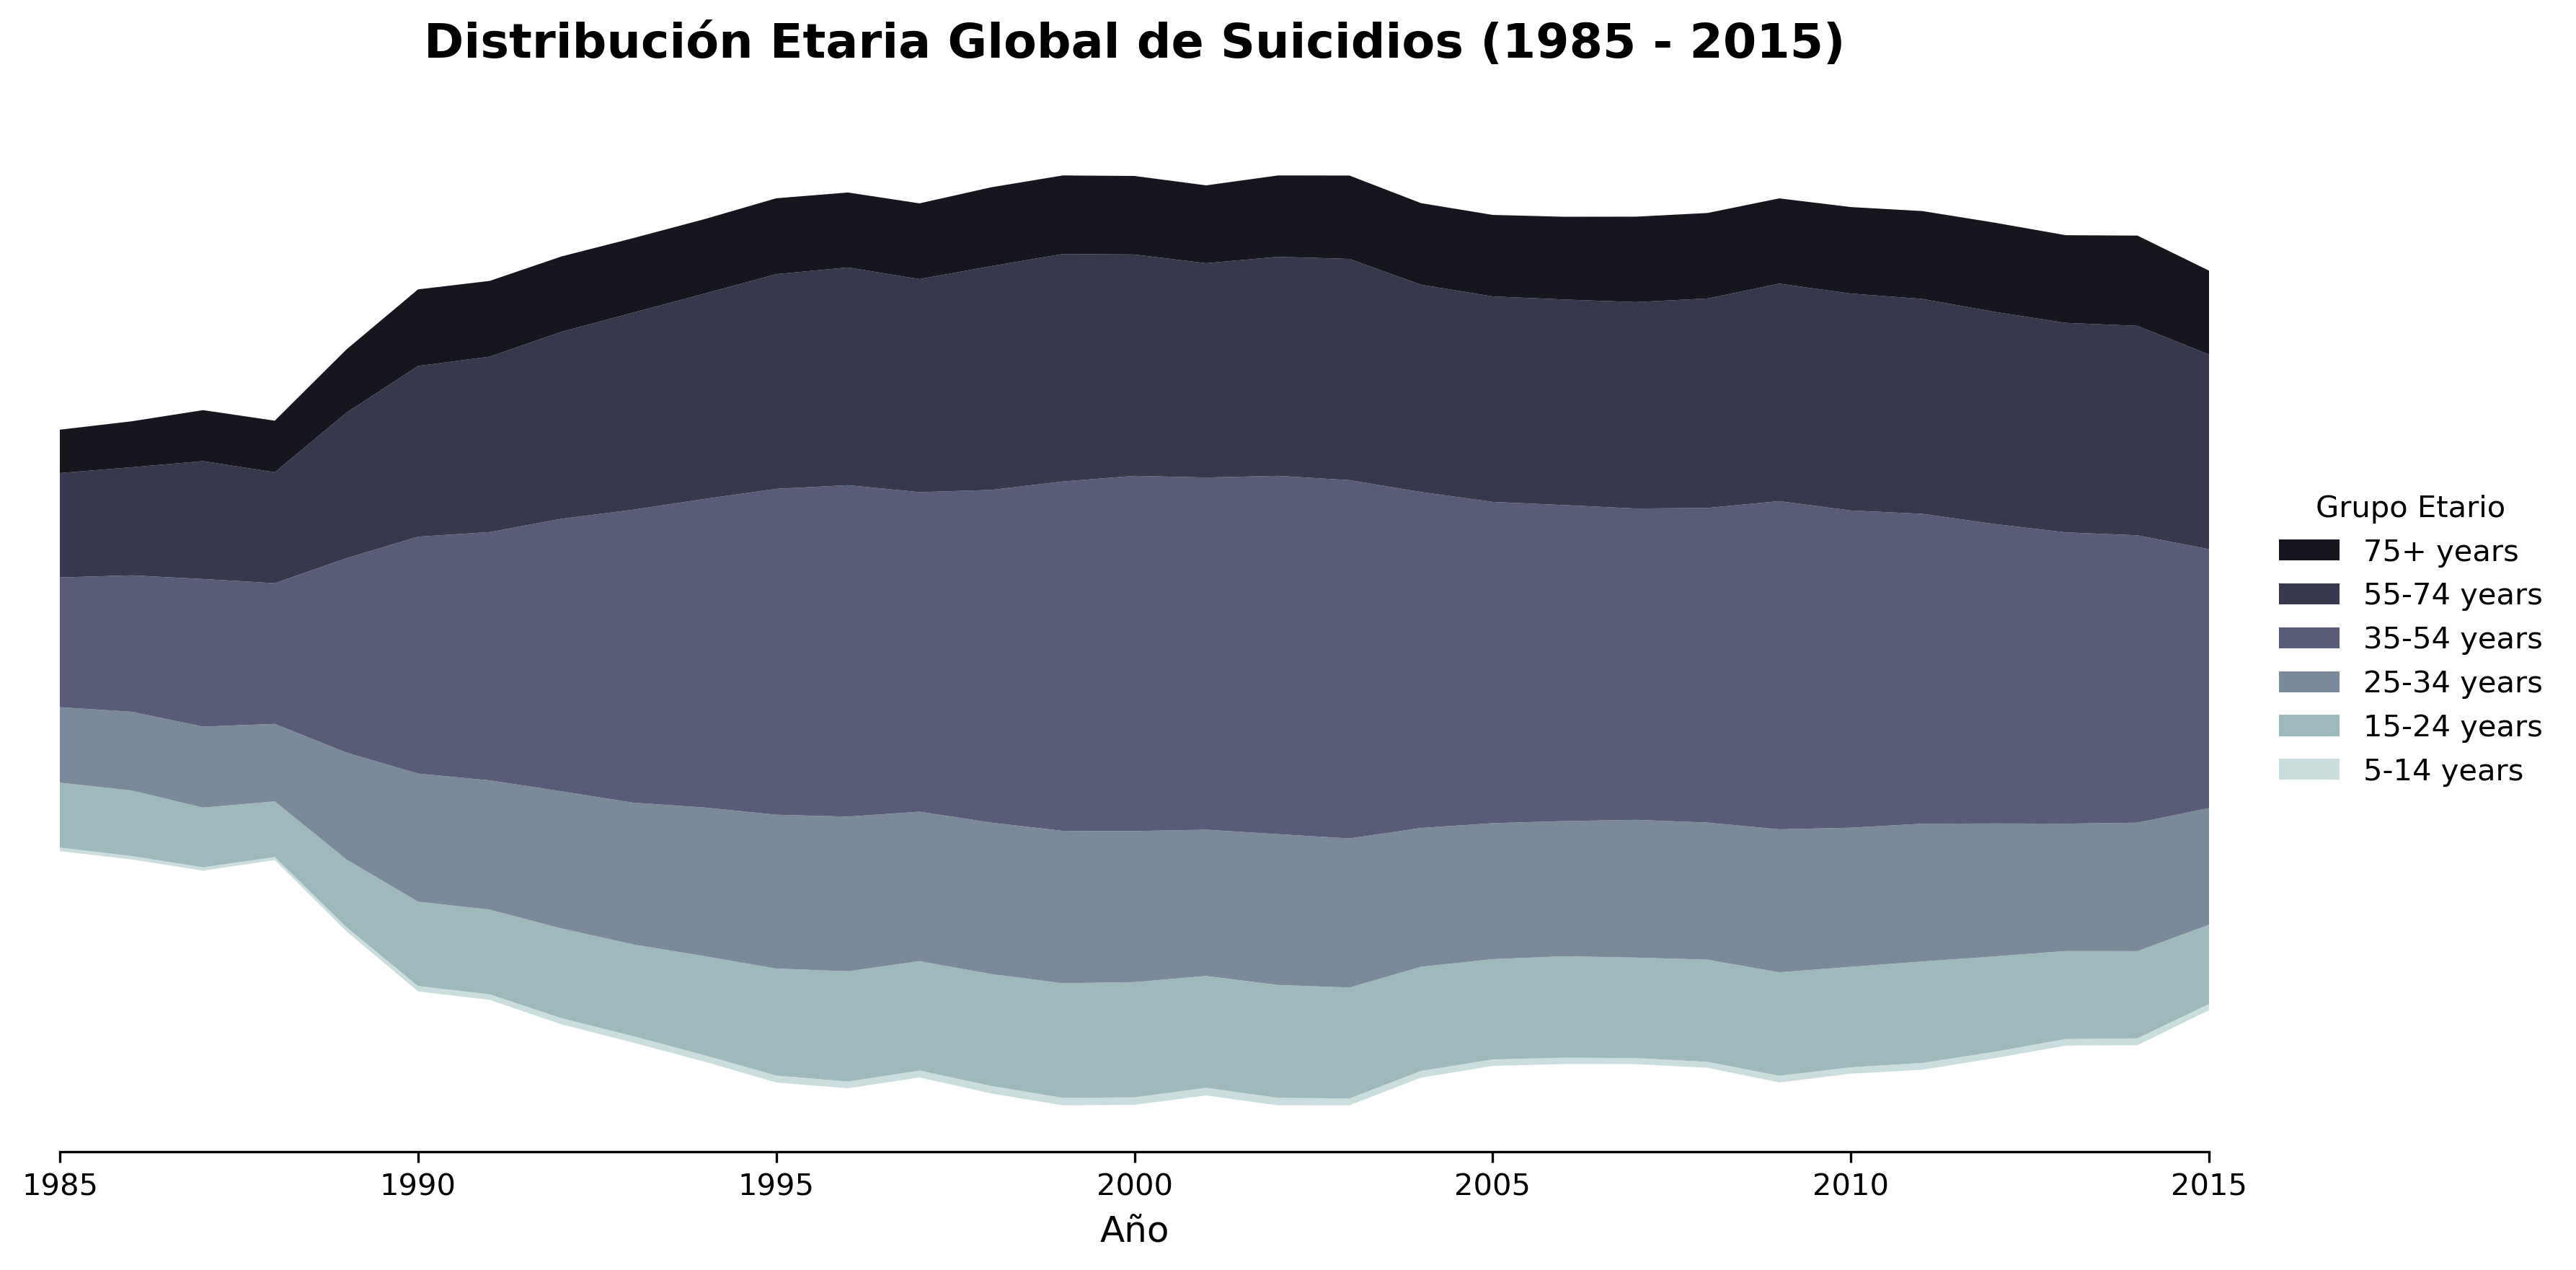
\includegraphics[width=0.85\textwidth]{figures/figure002.png}
  \caption{Distribución Etaria Global de Suicidios (1985 - 2015). Fuente: Kaggle -- Suicide Rates Overview 1985--2016.}
  \label{fig:figure002}
\end{figure}

\subsubsection*{Conclusiones}

\begin{itemize}
    \item El mayor volumen de casos recae de forma sostenida en la población adulta, específicamente en las franjas de 35-54 años y 55-74 años.
    \item Aunque los mayores de 75 años son una parte pequeña de la población mundial, su franja en el gráfico destaca bastante. Esto significa que la proporción de suicidios en la tercera edad es preocupantemente alta.
    \item El ensanchamiento simultáneo de todas las franjas alrededor del año 2000 demuestra que el aumento de casos en esa época afectó de manera transversal a todas las generaciones.
\end{itemize}

% ─────────────────────────────────────────────────────────────────────────────
\section{Trabajo individual -- Integrante 2: Andrés Águila}

\subsection{Criterios seleccionados}

\begin{enumerate}
  \item \textbf{Criterio A:} [Describir brevemente el criterio].
  \item \textbf{Criterio B:} [Describir brevemente el criterio].
\end{enumerate}

\subsection{Justificación de los criterios}

[Explicar por qué se eligieron estos criterios y cómo contribuyen al macrotema.]

\subsection{Visualización 3}

\begin{figure}[H]
  \centering
  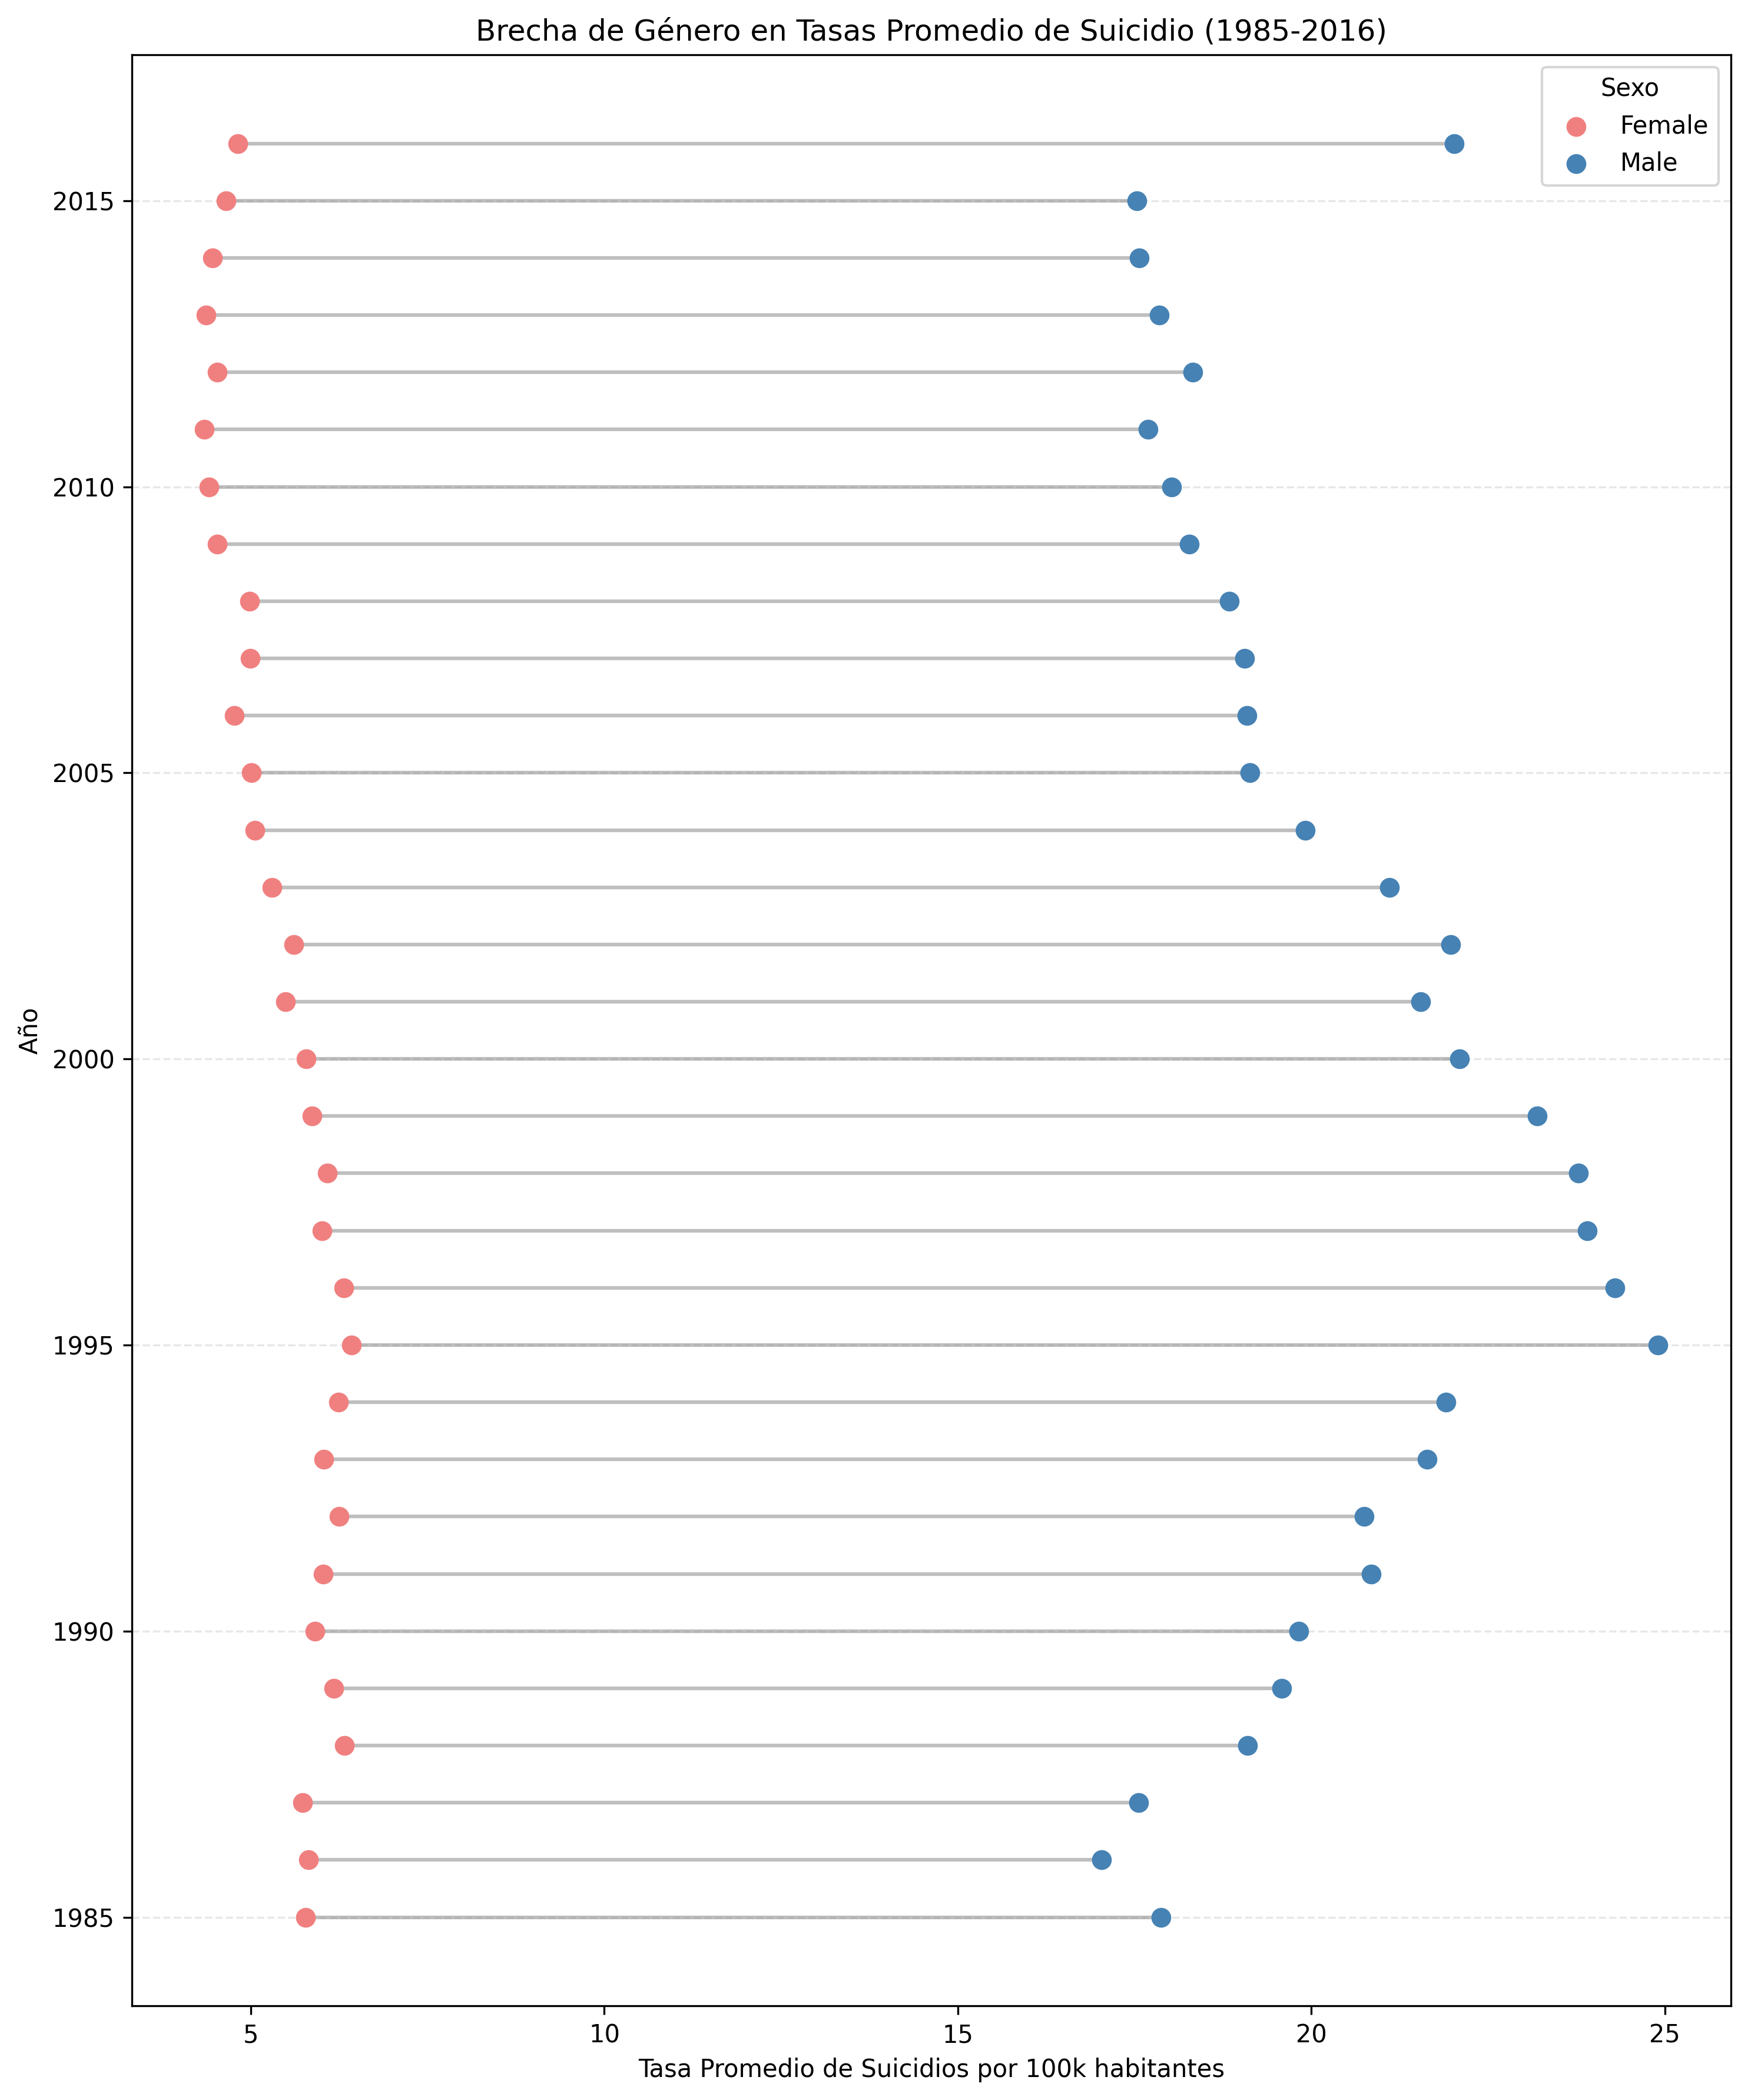
\includegraphics[width=0.85\textwidth]{figures/figure003.png}
  \caption{Evolución de la Cantidad Global de Suicidios (1985 - 2015). Fuente: Kaggle -- Suicide Rates Overview 1985--2016.}
  \label{fig:figure003}
\end{figure}

\subsubsection*{Conclusiones}

[Redactar las conclusiones obtenidas a partir de la Visualización 3.]

\subsection{Visualización 4 (individual)}

\begin{figure}[H]
  \centering
  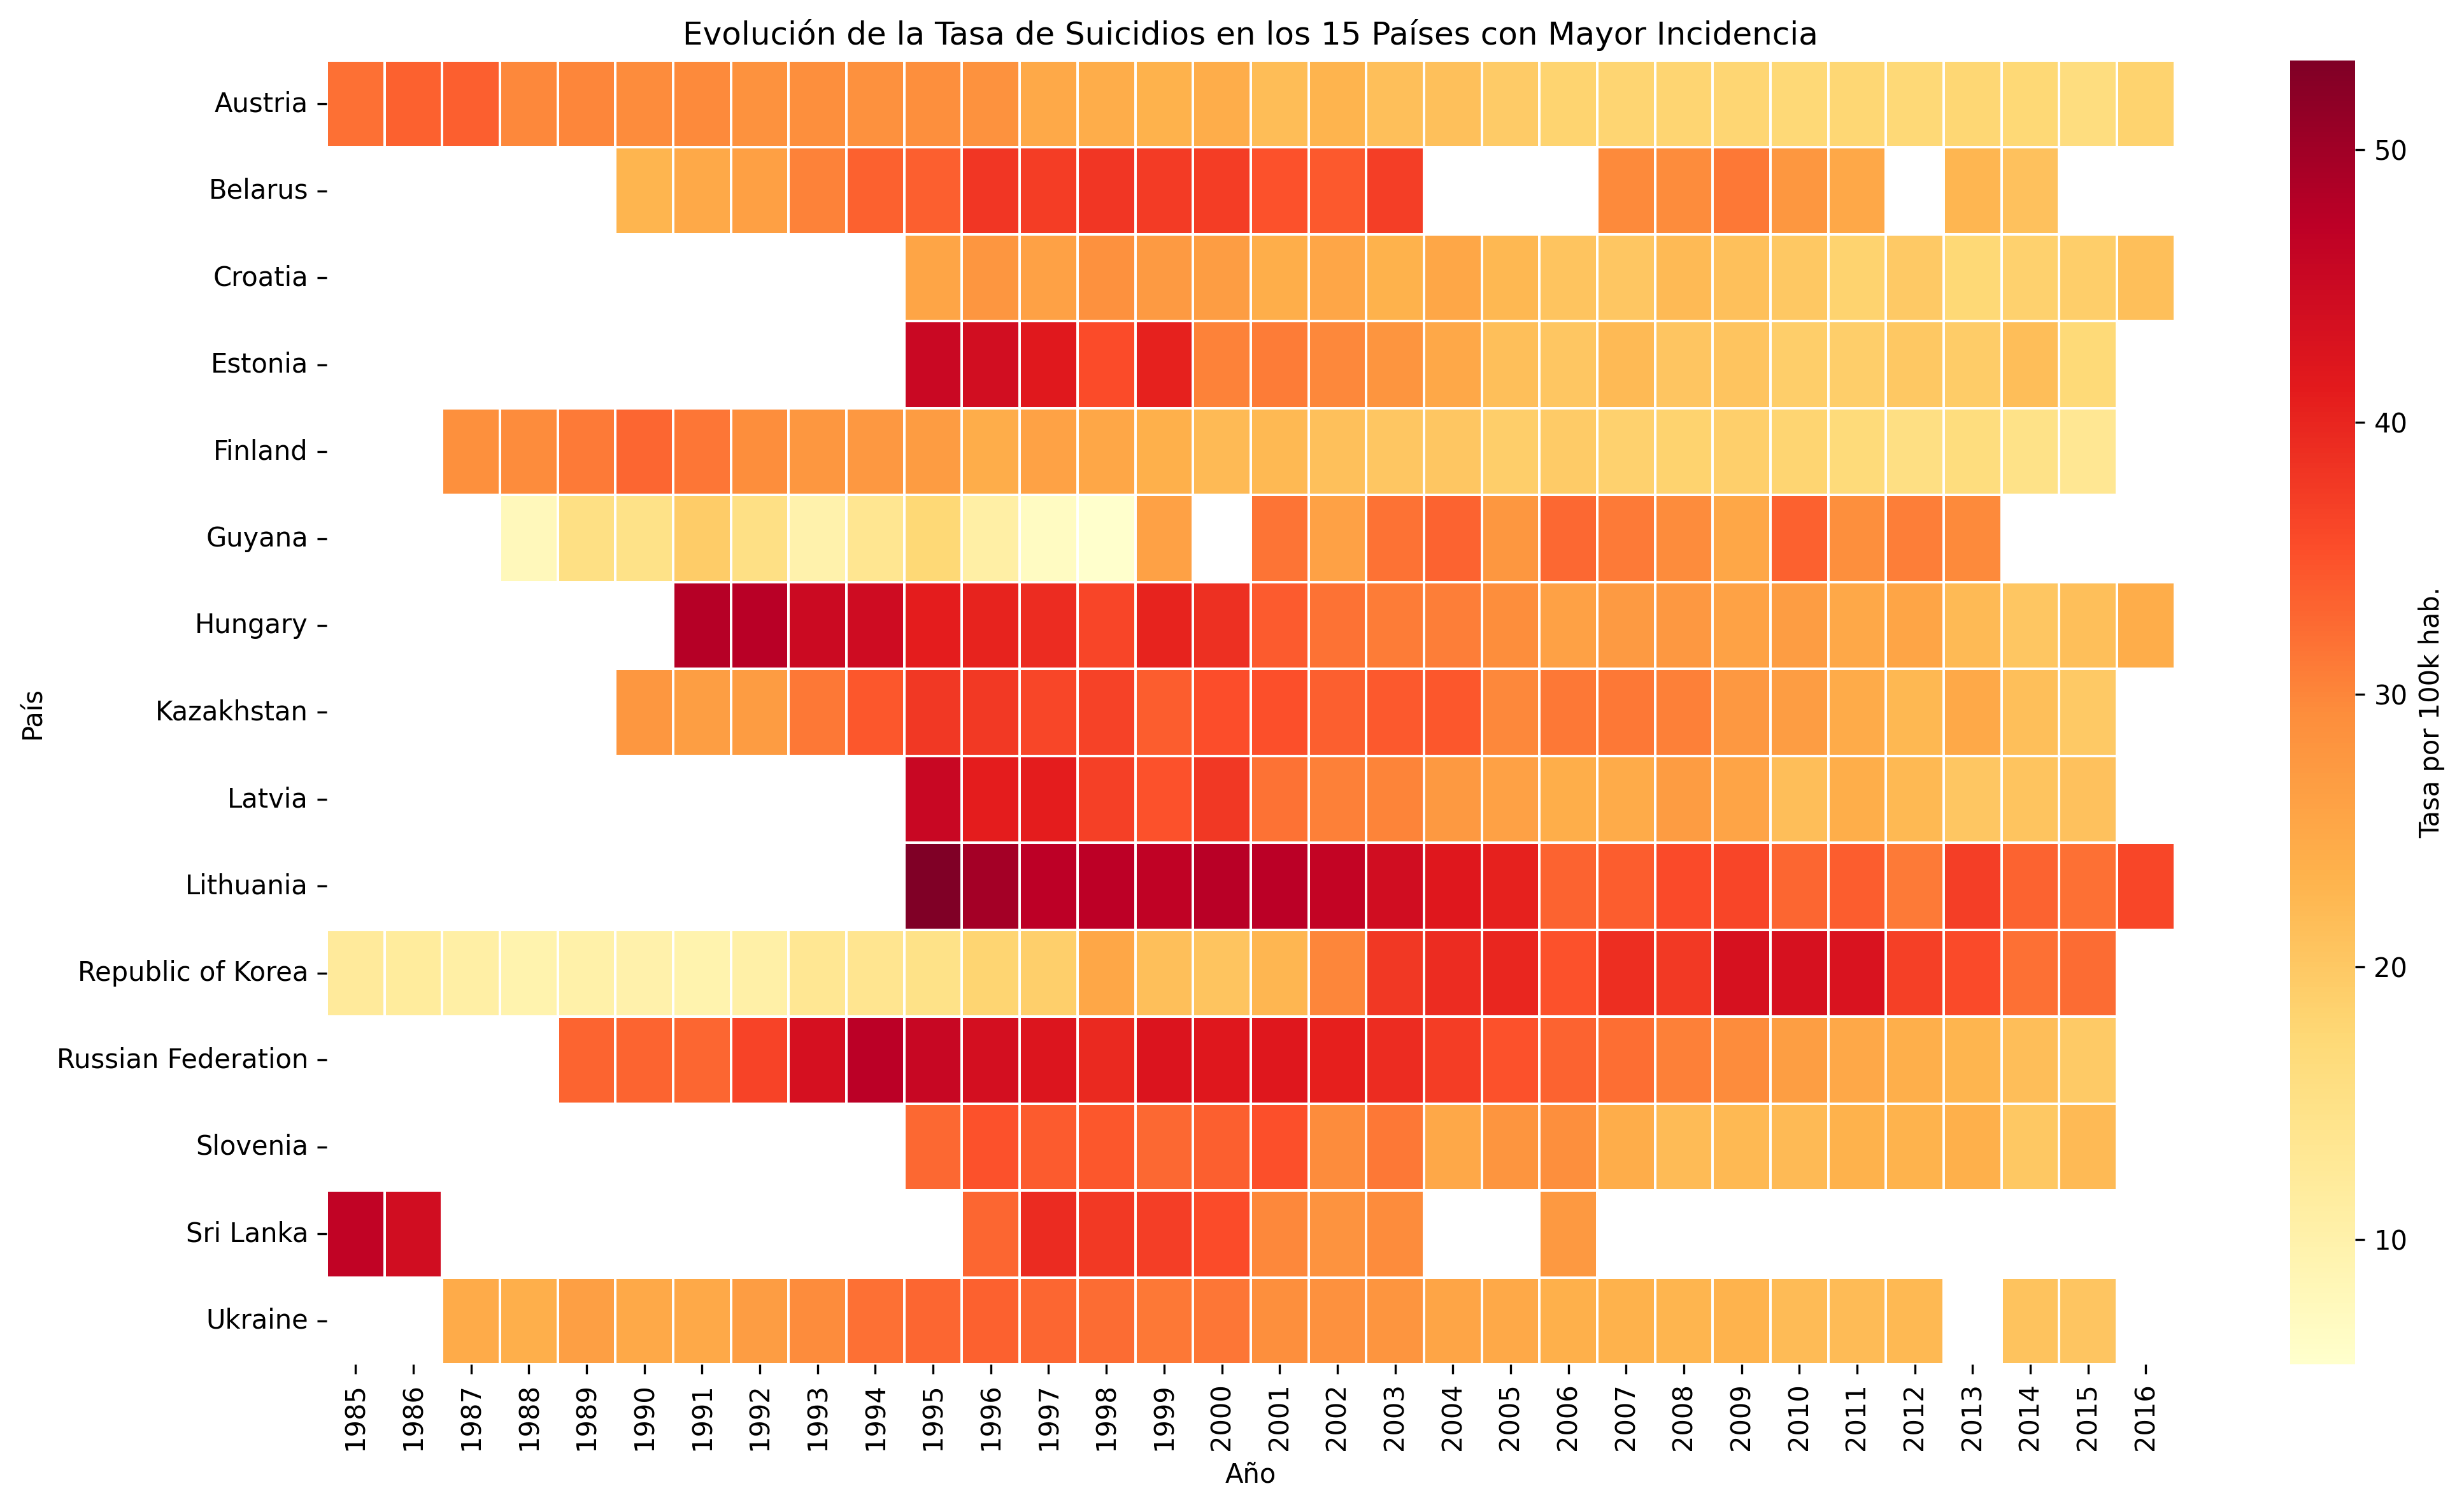
\includegraphics[width=0.85\textwidth]{figures/figure004.png}
  \caption{Evolución de la Cantidad Global de Suicidios (1985 - 2015). Fuente: Kaggle -- Suicide Rates Overview 1985--2016.}
  \label{fig:figure004}
\end{figure}

\subsubsection*{Conclusiones}

[Redactar las conclusiones obtenidas a partir de esta visualización.]

% ─────────────────────────────────────────────────────────────────────────────
\section{Trabajo grupal -- Visualización con IA generativa}

\subsection{Prompt utilizado}

\begin{lstlisting}[basicstyle=\small\ttfamily, breaklines=true, frame=single, mathescape=false]
Actúa como un periodista de datos y experto en visualización en Python. Cuento con un dataset sobre suicidios a nivel mundial (guardado localmente como 'suicide_dataset.csv') con las siguientes variables: country, year, sex, age, suicides_no, population, suicides/100k pop, HDI for year, gdp_per_capita ($). En caso de necesitar información original, el dataset se puede encontrar en: https://www.kaggle.com/datasets/russellyates88/suicide-rates-overview-1985-to-2016

Nuestro informe de investigación sigue este hilo conductor:

- Criterio A: Evolución de la cantidad global de suicidios (Gráfico de código de barras).

- Criterio B: Distribución etaria a lo largo del tiempo (Streamline plot).

- Criterio C: Brecha de género en tasas de suicidio (Dumbbell plot).

- Criterio D: Evolución de las tasas en los 15 países de mayor incidencia (Heatmap).

Eres el encargado de diseñar y programar el Criterio E (Visualización Grupal). Este criterio debe cerrar el hilo conductor evaluando la relación entre el nivel económico/desarrollo de los países (usando gdp_per_capita o HDI) y sus tasas de suicidio (suicides/100k pop).

Reglas estrictas:

- Prohibido usar gráficos de uso común (barras, dispersión, líneas, torta, etc.) y prohibido repetir los gráficos ya mencionados (código de barras, streamline, dumbbell, heatmap). Propón un gráfico estadístico avanzado y poco común.

- Escribe el código en Python (pandas, matplotlib, seaborn, u otras librerías necesarias) para generar el gráfico. Asume que el archivo 'suicide_dataset.csv' está en el mismo directorio. El código no debe tener emojis y debe tener comentarios mínimos.

- Redacta la justificación metodológica de este criterio y 3 conclusiones periodísticas clave a partir de esta visualización para incluirlas en el informe formal.
\end{lstlisting}

\subsection{Herramienta utilizada}

Se utilizó un modelo agéntico impulsado por Claude Opus 4.6 (Thinking) via Antigravity. Una vez recibido el prompt, el agente desarrolló su propio código en python y generó la visualización. A partir de esta realizó su propio análisis y conclusiones, los cuales se detallan en la siguiente sección.

\subsection{Código generado}

[Describir brevemente el código producido por la IA. Adjuntar el código completo en el repositorio
de GitHub y referenciarlo aquí.]

\subsection{Modificaciones realizadas}

[Detallar qué cambios se hicieron al código generado para obtener la visualización final, o
indicar que no fue necesario modificar nada.]

\subsection{Visualización grupal}


\begin{figure}[H]
  \centering
  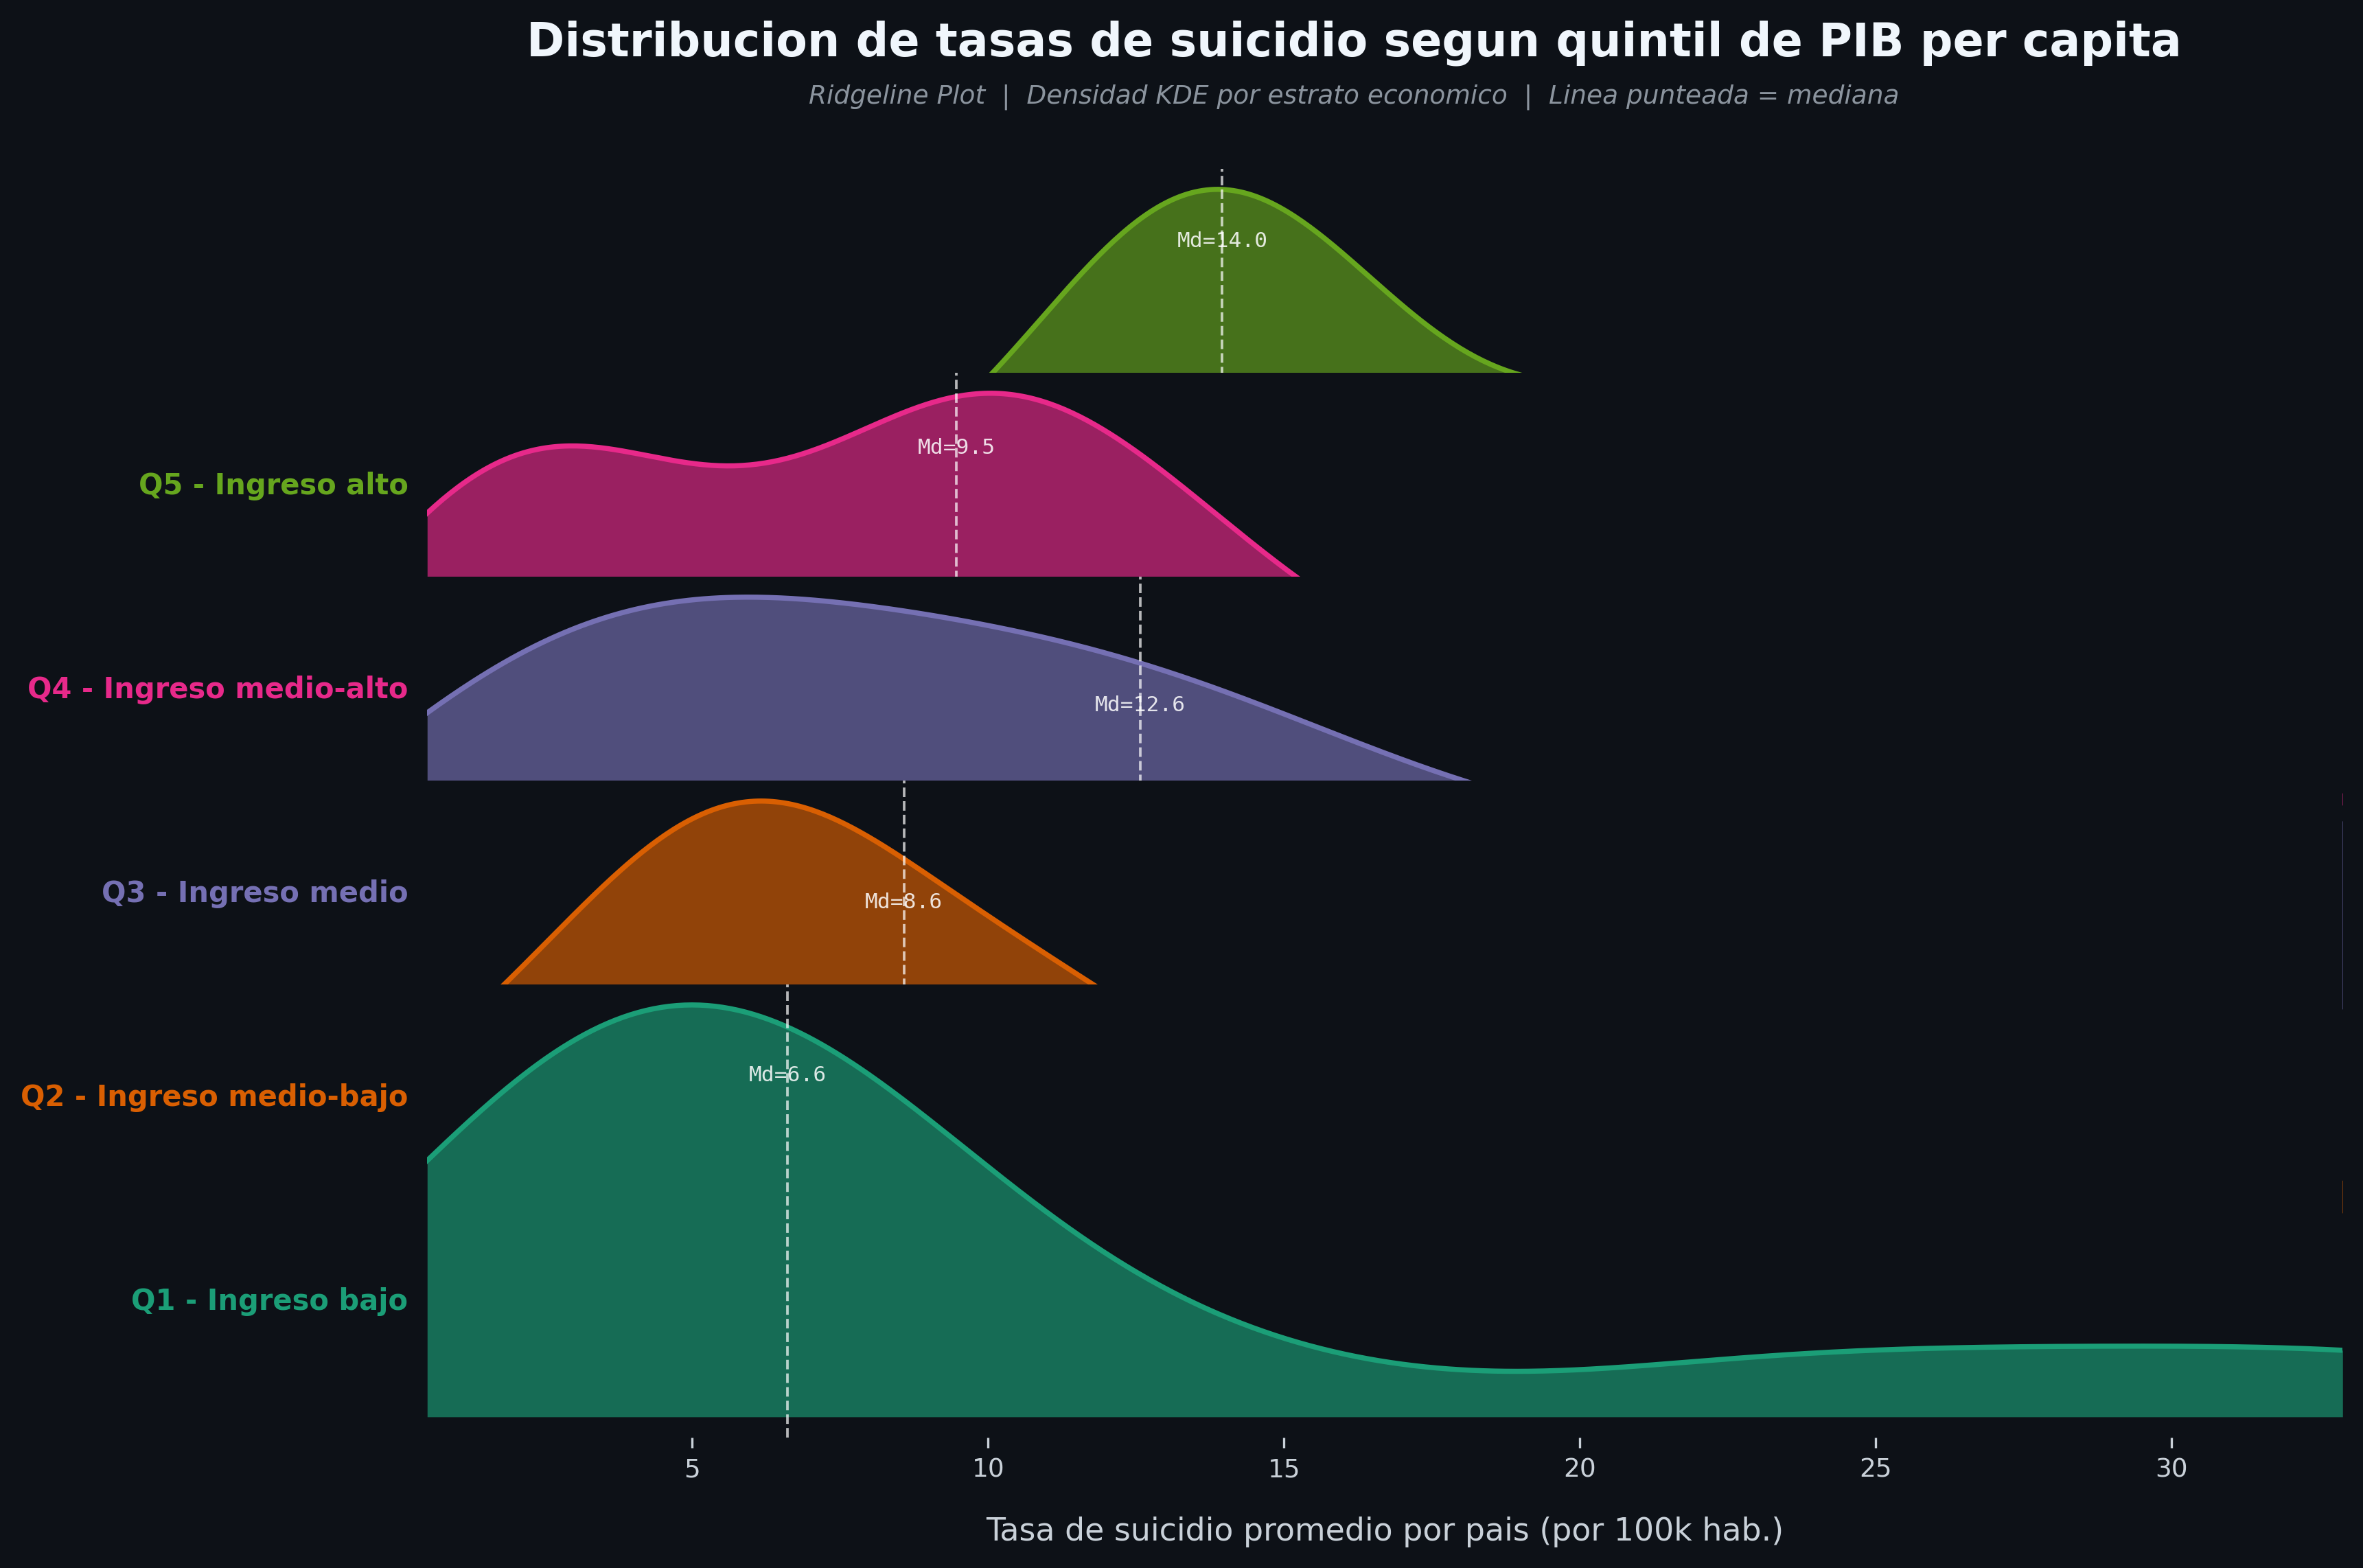
\includegraphics[width=0.85\textwidth]{figures/figure005.png}
  \caption{Evolución de la Cantidad Global de Suicidios (1985 - 2015). Fuente: Kaggle -- Suicide Rates Overview 1985--2016.}
  \label{fig:figure005}
\end{figure}

\subsubsection*{Conclusiones}

[Redactar las conclusiones grupales obtenidas de esta visualización y cómo se conecta con el
hilo conductor del trabajo.]

% ─────────────────────────────────────────────────────────────────────────────
\section{Conclusiones generales}

[Párrafo o dos que integren los hallazgos de todas las visualizaciones y los vinculen al
macrotema. Debe quedar claro el hilo conductor del trabajo.]

% ─────────────────────────────────────────────────────────────────────────────
\section{Repositorio de GitHub}

El código fuente de todas las visualizaciones se encuentra disponible en el siguiente repositorio:

\begin{center}
  \href{https://github.com/USUARIO/REPOSITORIO}{\texttt{https://github.com/USUARIO/REPOSITORIO}}
\end{center}

La estructura del repositorio es la siguiente:

\begin{verbatim}
  /
  |-- datos/
  |   |-- README.md          # Origen y descripción de los datos
  |-- codigo/
  |   |-- integrante1/       # Scripts de NOMBRE 1
  |   |-- integrante2/       # Scripts de NOMBRE 2
  |-- README.md
\end{verbatim}

% ─────────────────────────────────────────────────────────────────────────────

\end{document}
